%%=============================================================================
%% Puppetboard
%%=============================================================================

\chapter{\IfLanguageName{dutch}{Puppetboard}{Puppetboard}}%
\label{ch:bijlage_puppetboard}

Afbeelding~\ref{fig:puppetboard-home} toont een voorbeeld van de startpagina van Puppetboard.
Hier krijgt men een beknopt overzicht van het aantal nodes dat door Puppet wordt beheerd en de totale hoeveelheid resources die wordt beheerd.
Ook kan men zien hoeveel runs zijn mislukt en hoeveel succesvol waren.
Onder de grafieken bevindt zich een lijst van servers waarop Puppet recentelijk een run heeft uitgevoerd om de gedefinieerde configuratie toe te passen.

\begin{figure}[h!]
    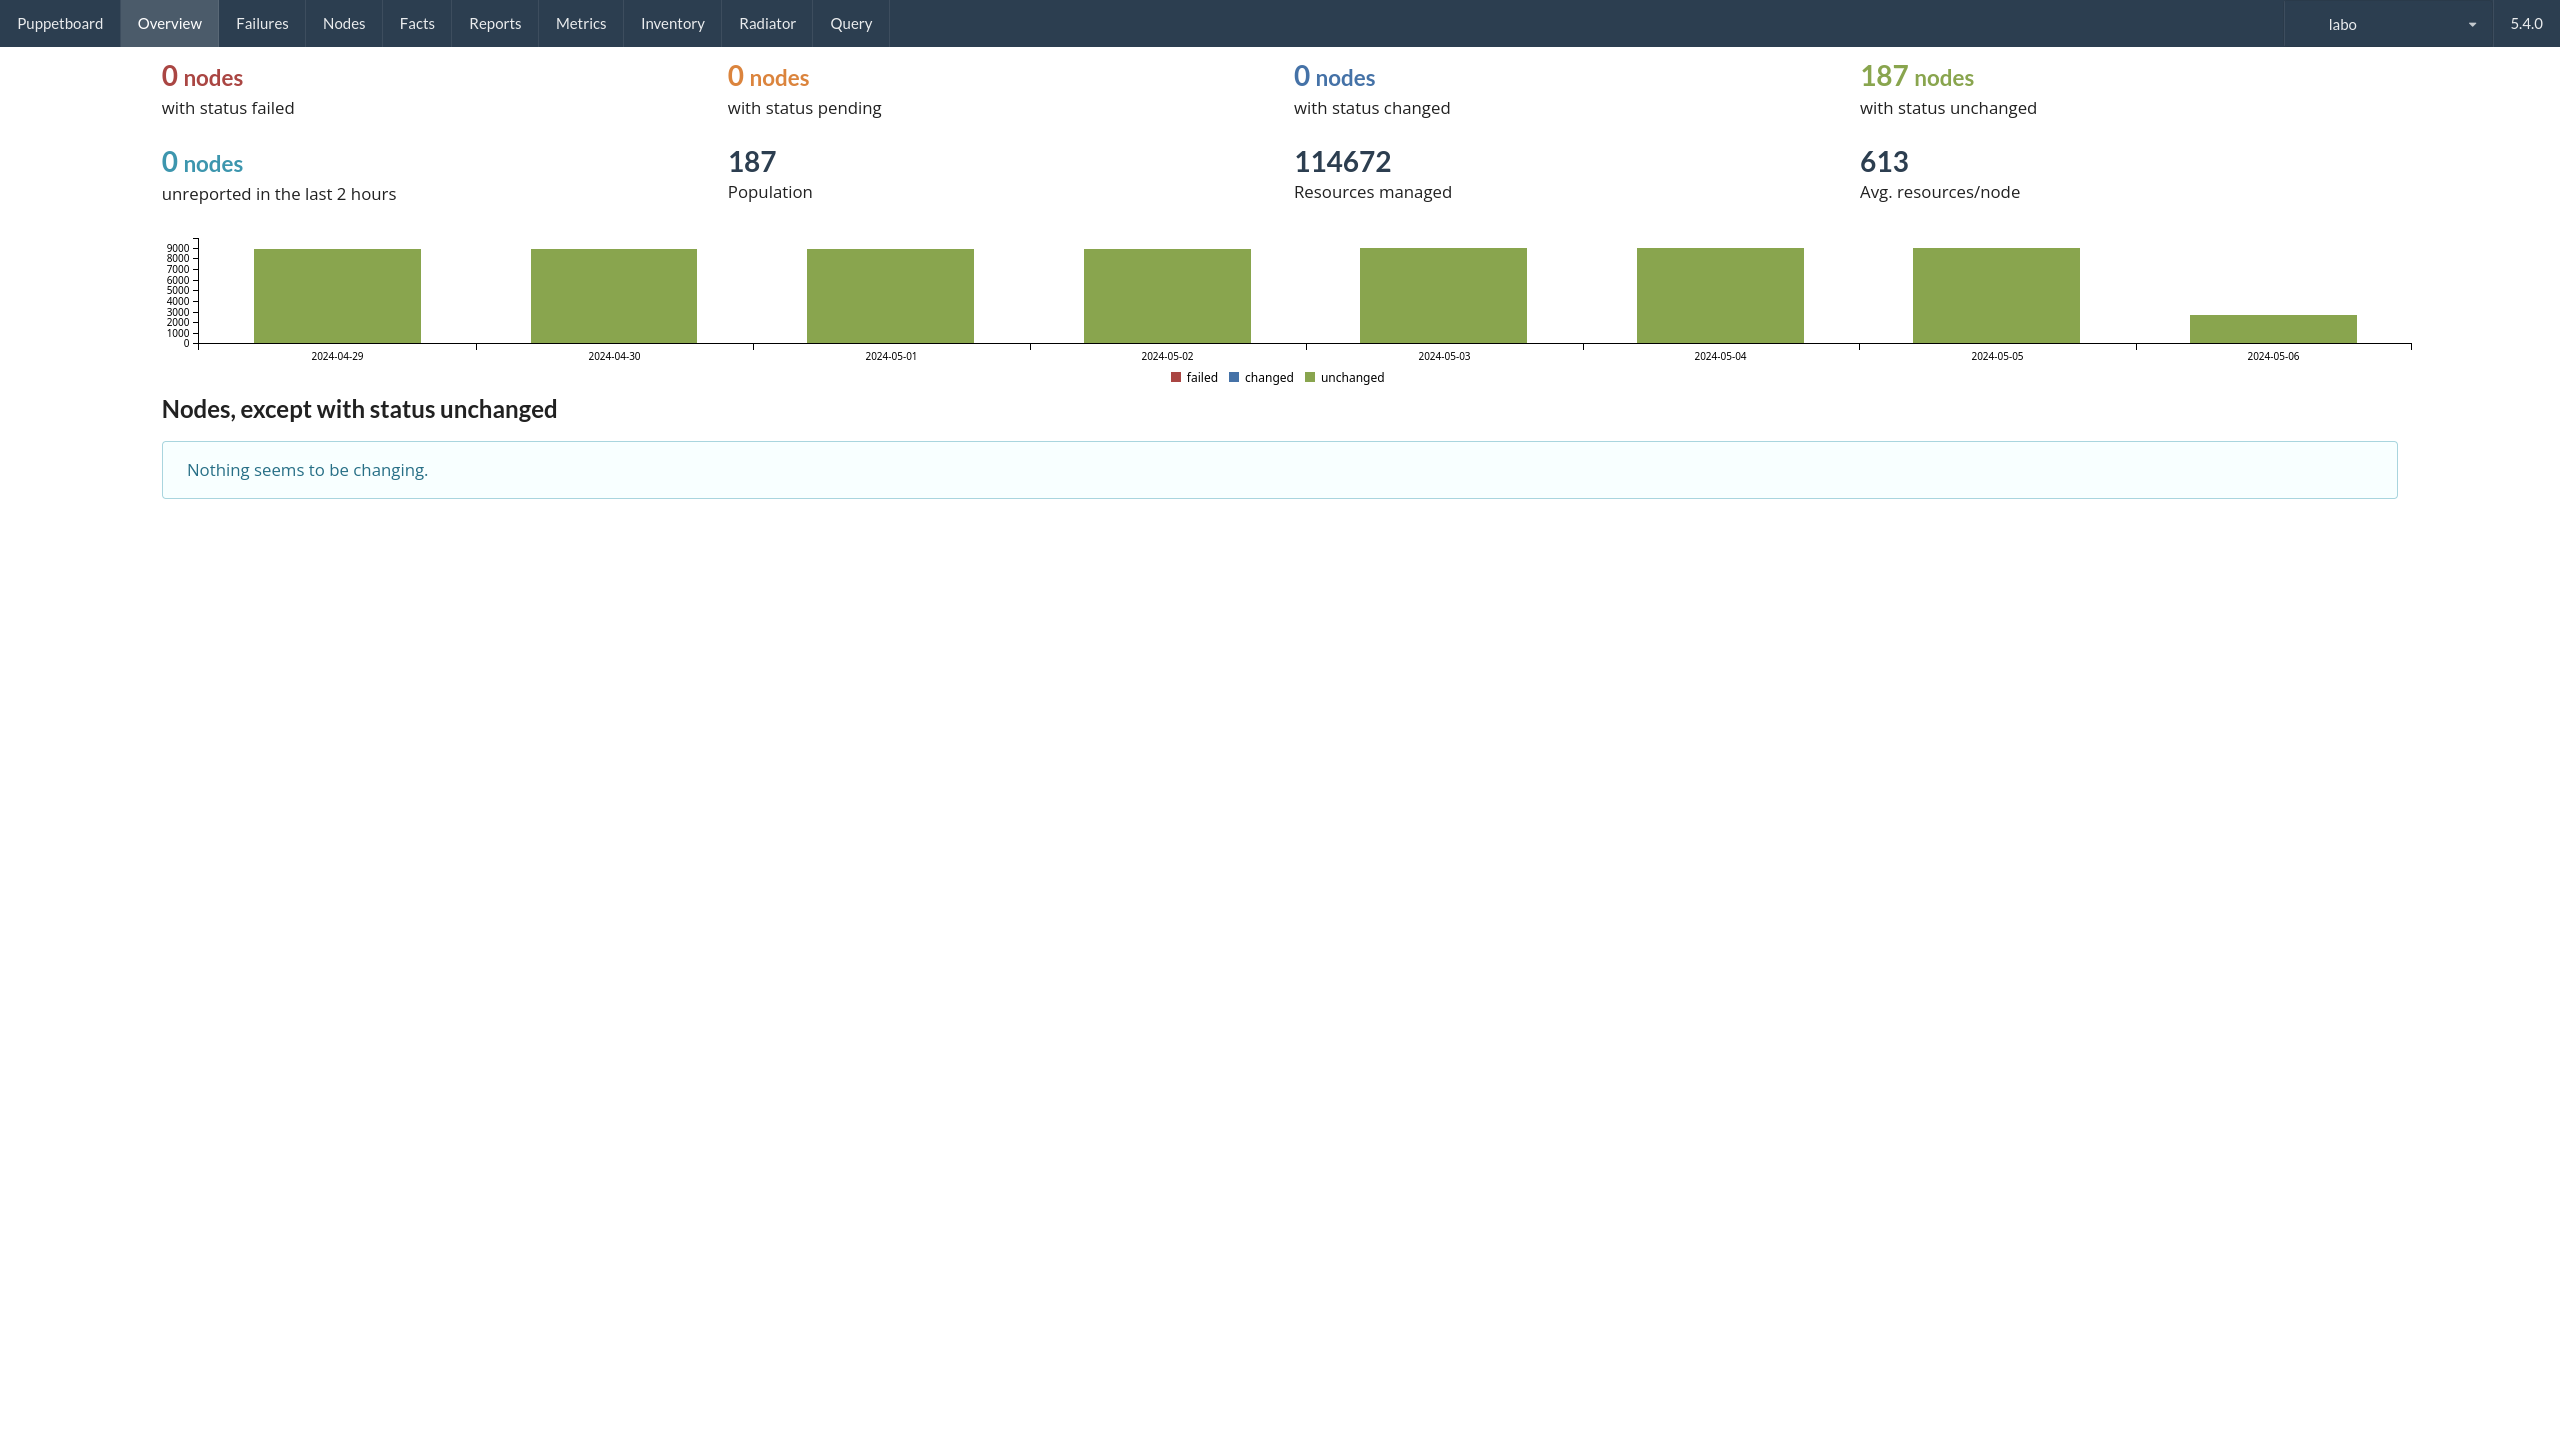
\includegraphics[width=\textwidth]
    {./graphics/state-of-the-art/puppetboard/puppetboard-home.png}
    \caption[Puppetboard startpagina.]{\label{fig:puppetboard-home}Voorbeeld van de Puppetboard startpagina. (Deze schermafbeelding werd genomen bij Federale Pensioendienst (FPD) met toestemming, gedurende persoonlijke stage.)}
\end{figure}

Afbeelding~\ref{fig:puppetboard-inventory} toont een overzicht van alle nodes die door Puppet worden beheerd.
Alsook wanneer de laatste run was en of deze succesvol was.

\begin{figure}[h!]
    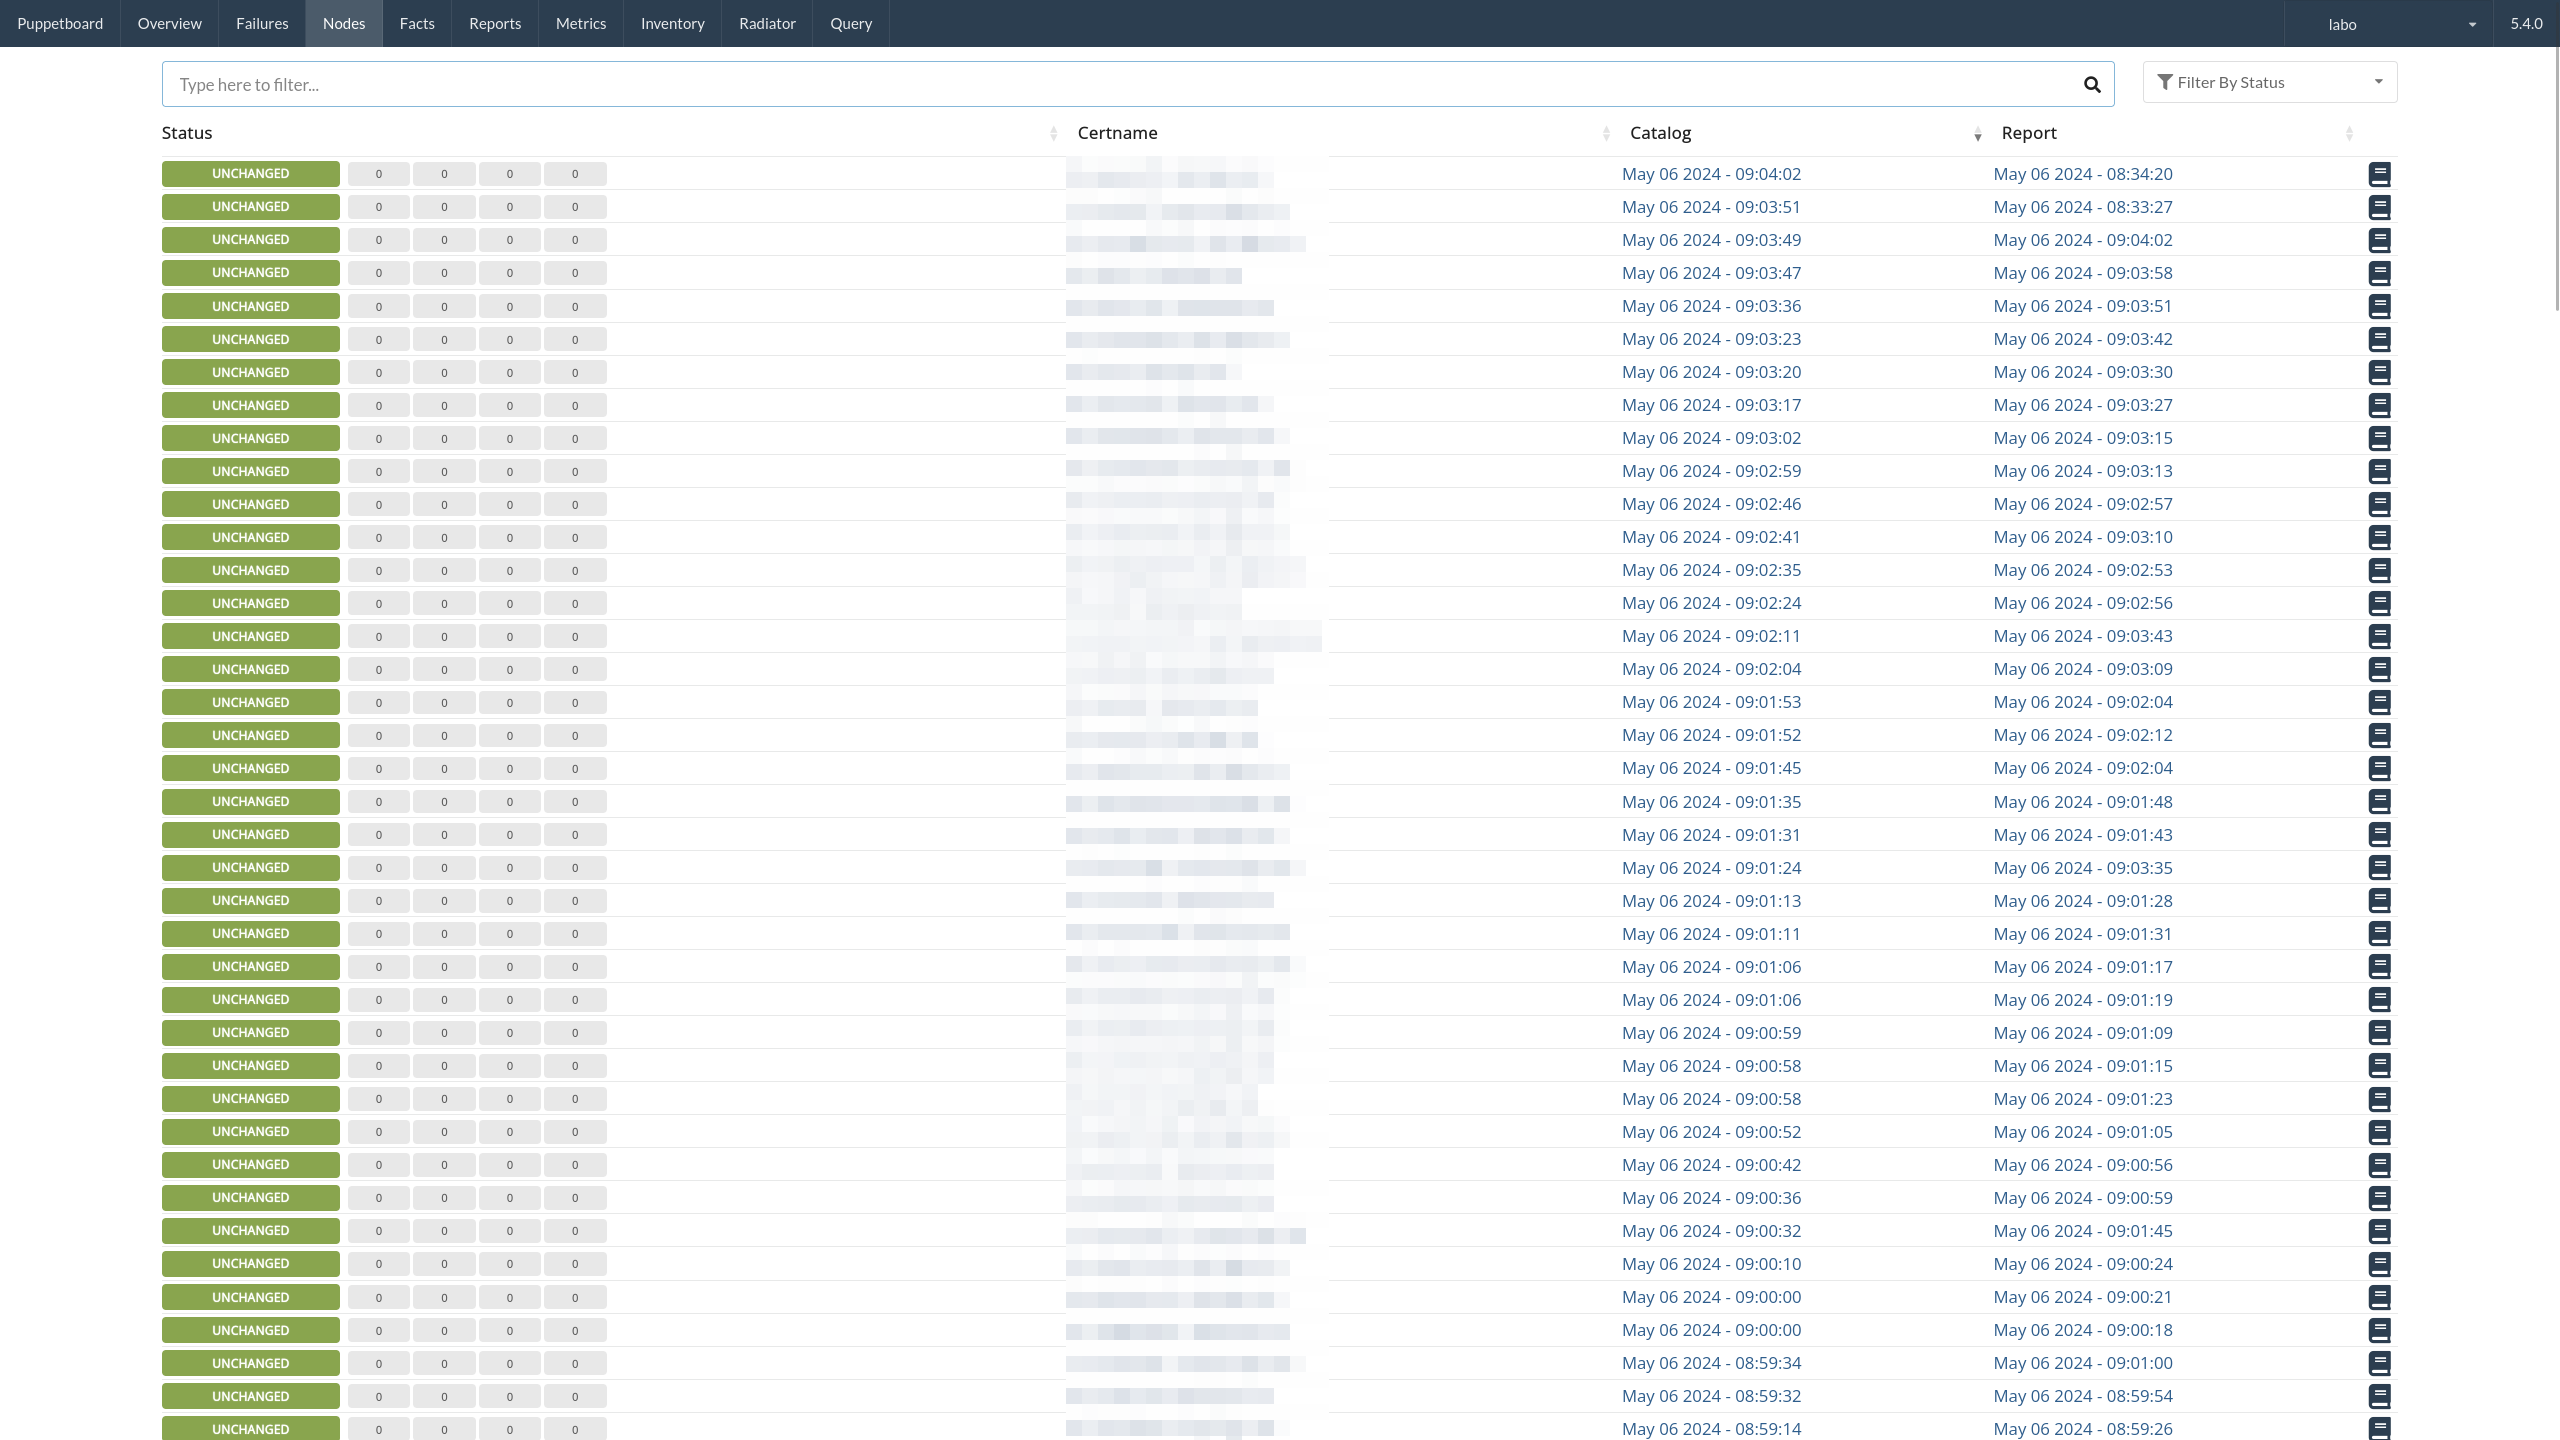
\includegraphics[width=\textwidth]
    {./graphics/state-of-the-art/puppetboard/puppetboard-hosts.png}
    \caption[Puppetboard inventaris van nodes.]{\label{fig:puppetboard-inventory}Voorbeeld van de Puppetboard waar men alle nodes van het inventaris kan zien. (Deze schermafbeelding werd genomen bij Federale Pensioendienst (FPD) met toestemming, gedurende persoonlijke stage.)}
\end{figure}

Afbeelding~\ref{fig:puppetboard-example-4} toont een lijst van verschillende nodes die door Puppet worden beheerd.
Men kan de hostname, IP-adres, besturingssysteem, CPU-arhitectuur, kernelversie en de Puppet-agent versie zien.

\begin{figure}[h!]
    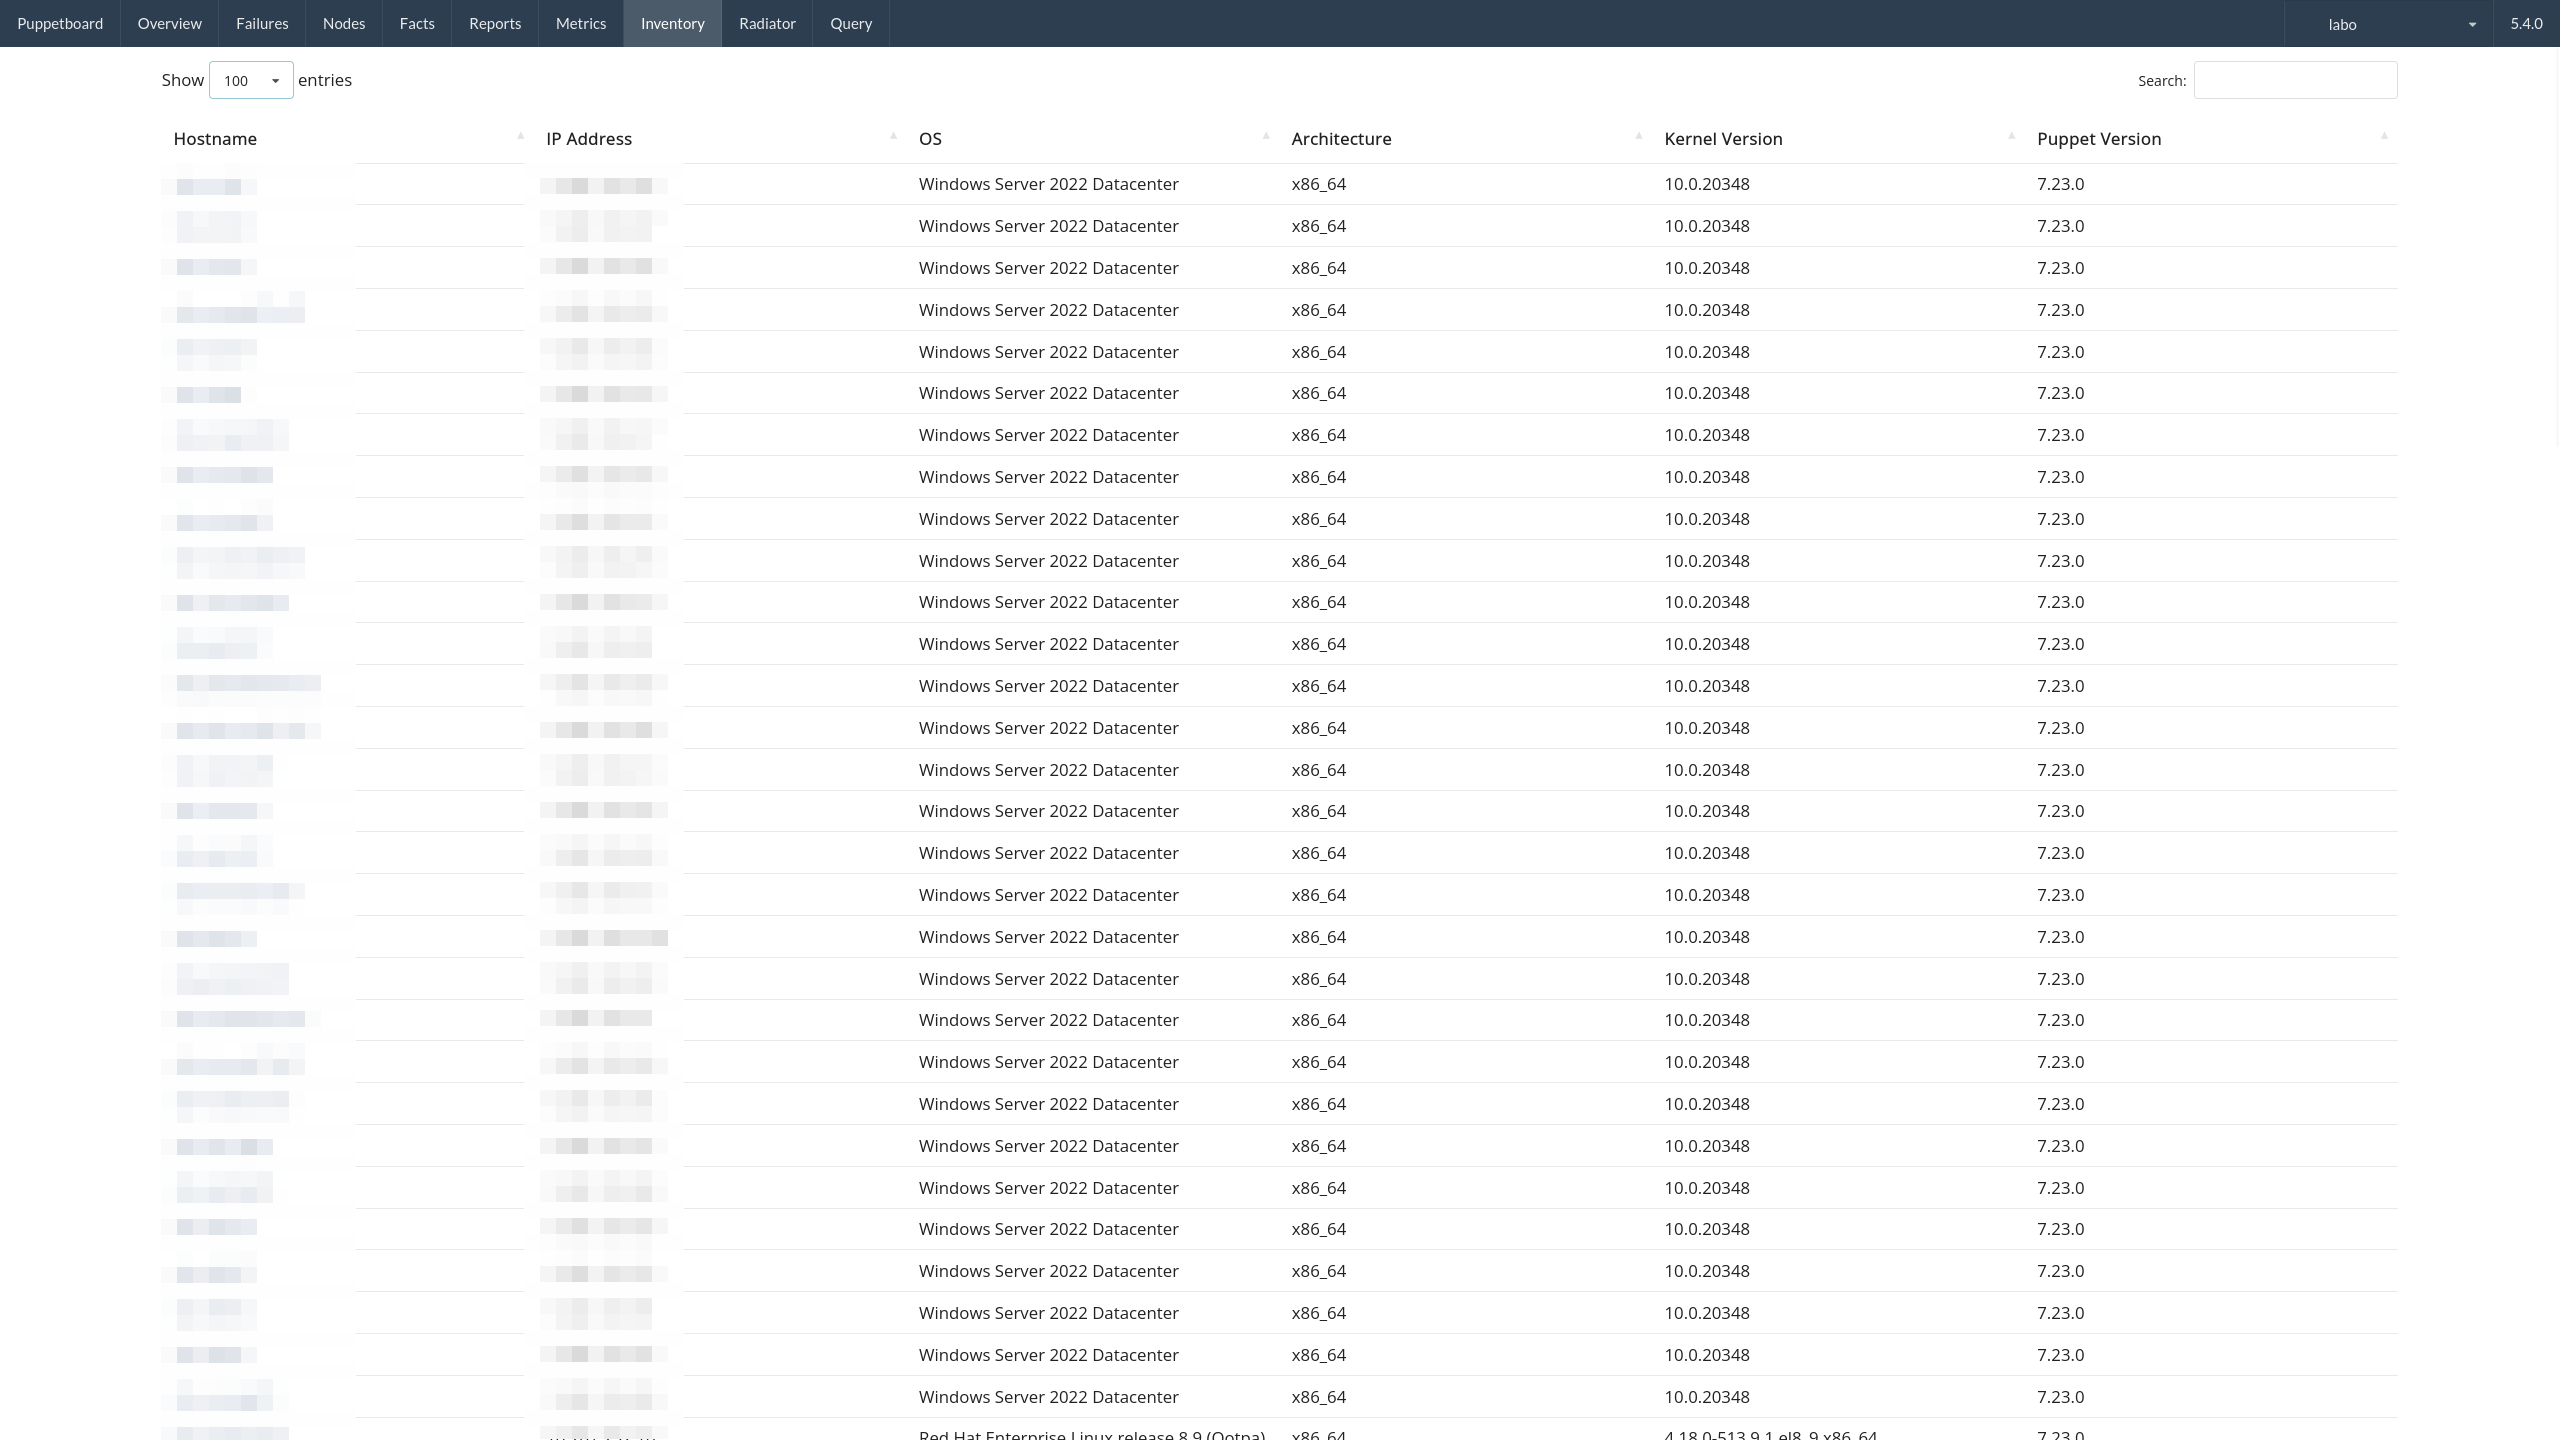
\includegraphics[width=\textwidth]
    {./graphics/state-of-the-art/puppetboard/puppetboard-inventory.png}
    \caption[Basisinformatie op Puppetboard.]{\label{fig:puppetboard-example-4}Voorbeeld van de Puppetboard waar men basis informatie over het systeem kan vinden. (Deze schermafbeelding werd genomen bij Federale Pensioendienst (FPD) met toestemming, gedurende persoonlijke stage.)}
\end{figure}
